% Für Bindekorrektur als optionales Argument "BCORfaktormitmaßeinheit", dann
% sieht auch Option "twoside" vernünftig aus
% Näheres zu "scrartcl" bzw. "scrreprt" und "scrbook" siehe KOMA-Skript Doku
\documentclass[12pt,a4paper,titlepage,headinclude,bibtotoc]{scrartcl}


%---- Allgemeine Layout Einstellungen ------------------------------------------

% Für Kopf und Fußzeilen, siehe auch KOMA-Skript Doku
\usepackage[komastyle]{scrpage2}
\pagestyle{scrheadings}
\setheadsepline{0.5pt}[\color{black}]
\automark[section]{chapter}


%Einstellungen für Figuren- und Tabellenbeschriftungen
\setkomafont{captionlabel}{\sffamily\bfseries}
\setcapindent{0em}


%---- Weitere Pakete -----------------------------------------------------------
% Die Pakete sind alle in der TeX Live Distribution enthalten. Wichtige Adressen
% www.ctan.org, www.dante.de

% Sprachunterstützung
\usepackage[ngerman]{babel}

% Benutzung von Umlauten direkt im Text
% entweder "latin1" oder "utf8"
\usepackage[utf8]{inputenc}

% Pakete mit Mathesymbolen und zur Beseitigung von Schwächen der Mathe-Umgebung
\usepackage{latexsym,exscale,stmaryrd,amssymb,amsmath}

% Weitere Symbole
\usepackage[nointegrals]{wasysym}
\usepackage{eurosym}

% Anderes Literaturverzeichnisformat
%\usepackage[square,sort&compress]{natbib}

% Für Farbe
\usepackage{color}

% Zur Graphikausgabe
%Beipiel: \includegraphics[width=\textwidth]{grafik.png}
\usepackage{graphicx}

% Text umfließt Graphiken und Tabellen
% Beispiel:
% \begin{wrapfigure}[Zeilenanzahl]{"l" oder "r"}{breite}
%   \centering
%   \includegraphics[width=...]{grafik}
%   \caption{Beschriftung} 
%   \label{fig:grafik}
% \end{wrapfigure}
\usepackage{wrapfig}

% Mehrere Abbildungen nebeneinander
% Beispiel:
% \begin{figure}[htb]
%   \centering
%   \subfigure[Beschriftung 1\label{fig:label1}]
%   {\includegraphics[width=0.49\textwidth]{grafik1}}
%   \hfill
%   \subfigure[Beschriftung 2\label{fig:label2}]
%   {\includegraphics[width=0.49\textwidth]{grafik2}}
%   \caption{Beschriftung allgemein}
%   \label{fig:label-gesamt}
% \end{figure}
\usepackage{subfigure}

% Caption neben Abbildung
% Beispiel:
% \sidecaptionvpos{figure}{"c" oder "t" oder "b"}
% \begin{SCfigure}[rel. Breite (normalerweise = 1)][hbt]
%   \centering
%   \includegraphics[width=0.5\textwidth]{grafik.png}
%   \caption{Beschreibung}
%   \label{fig:}
% \end{SCfigure}
\usepackage{sidecap}

% Befehl für "Entspricht"-Zeichen
\newcommand{\corresponds}{\ensuremath{\mathrel{\widehat{=}}}}
% Befehl für Errorfunction
\newcommand{\erf}[1]{\text{ erf}\ensuremath{\left( #1 \right)}}

%Fußnoten zwingend auf diese Seite setzen
\interfootnotelinepenalty=1000

%Für chemische Formeln (von www.dante.de)
%% Anpassung an LaTeX(2e) von Bernd Raichle
\makeatletter
\DeclareRobustCommand{\chemical}[1]{%
  {\(\m@th
   \edef\resetfontdimens{\noexpand\)%
       \fontdimen16\textfont2=\the\fontdimen16\textfont2
       \fontdimen17\textfont2=\the\fontdimen17\textfont2\relax}%
   \fontdimen16\textfont2=2.7pt \fontdimen17\textfont2=2.7pt
   \mathrm{#1}%
   \resetfontdimens}}
\makeatother

%Honecker-Kasten mit $$\shadowbox{$xxxx$}$$
\usepackage{fancybox}

%SI-Package
\usepackage{siunitx}

%keine Einrückung, wenn Latex doppelte Leerzeile
\parindent0pt

%Bibliography \bibliography{literatur} und \cite{gerthsen}
%\usepackage{cite}
\usepackage{babelbib}
\selectbiblanguage{ngerman}

\begin{document}

\begin{titlepage}
\centering
\textsc{\Large Anfängerpraktikum der Fakultät für
  Physik,\\[1.5ex] Universität Göttingen}

\vspace*{3cm}

\rule{\textwidth}{1pt}\\[0.5cm]
{\huge \bfseries
  Versuch Elektronik\\[1.5ex]
  Protokoll}\\[0.5cm]
\rule{\textwidth}{1pt}

\vspace*{3cm}

\begin{Large}
\begin{tabular}{ll}
Praktikant: &  Michael Lohmann\\
 &  Felix Kurtz\\
% &  Kevin Lüdemann\\
% &  Skrollan Detzler\\
 E-Mail: & m.lohmann@stud.uni-goettingen.de\\
 &  felix.kurtz@stud.uni-goettingen.de\\
% &  kevin.luedemann@stud.uni-goettingen.de\\
% &  skrollan.detzler@stud.uni-goettingen.de\\
 Betreuer: & ***************************\\
 Versuchsdatum: & **************************.2014\\
\end{tabular}
\end{Large}

\vspace*{0.8cm}

\begin{Large}
\fbox{
  \begin{minipage}[t][2.5cm][t]{6cm} 
    Testat:
  \end{minipage}
}
\end{Large}

\end{titlepage}

\tableofcontents

\newpage

\section{Einleitung}
\label{sec:einleitung}
Dioden sind technische Bauelemente, die nur einen Stromfluss in eine Richtung zulassen.
Vakuum-Dioden sind die wohl einfachsten, wenn auch heutzutage nicht mehr die gebräuchlichsten.
Ihre wichtigsten Kennlinien zu vermessen, kann daher Erkenntnisse für komplexere Aufbauten, wie zum Beispiel Halbleiterdioden, liefern.

\cite{gerthsen}

\section{Theorie}
\label{sec:theorie}
Eine Vakuum-Diode besteht aus einem Kathode-Anode-Paar, welches in einem Vakuum-Behältnis eingelassen ist.
Die Kathode besteht aus einer Glühlampe, welche regelbar beheizt werden kann.
\subsection{Austrittsarbeit der Elektronen}
Die Elektronen benötigen eine gewisse Energie um aus dem Draht auszutreten und zur Anode zu gelangen.
Sie wird dafür benötigt, sich aus dem positiv geladenen Gitter des Drahtes herauszulösen.
Diese Energie ist jedoch relativ hoch, so dass bei den hier verwendeten Spannungen kein Strom zu messen sein sollte.
Da die Kathode jedoch beheizt wird, bekommen die Elektronen im Draht eine thermische (und damit kinetische) Energie.
Dies ist auch der Grund, warum die Vakuum-Diode einen Elektronenfluss von der Anode zur Kathode verhindert.
Nicht alle Elektronen sind jedoch gleich schnell, so dass einige mehr kinetische besitzen als andere.
Die Verteilung der Geschwindigkeiten basiert auf der \textsc{Fermi}-Verteilung.
Der sich so ergebende Strom verhält sich nach der \textsc{Richardson}\emph{-Gleichung}:
\begin{align}
	j_R=A_R\cdot T^{2}\cdot \exp\left(-\frac{W_A}{k_BT}\right)\label{eq:richardson}\; .
\end{align}
Wobei $A_R\approx \SI{6e-3}{\ampere\meter^{-2}\kelvin^{-2}}$ die Richardson-Konstante darstellt.
Sie ist für alle reinen Metalle etwa gleich.
Zur Veringerung der Austrittsarbeit $W_A$ können Metalle mit Alkalimetallen oder Barium-Oxid überzogen werden, da diese eine geringere besitzen.


                                                                                                                                                                      
\section{Durchführung}
\label{sec:durchfuehrung}

\section{Auswertung}
\label{sec:auswertung}
\begin{figure}
	% GNUPLOT: LaTeX picture with Postscript
\begingroup
  \makeatletter
  \providecommand\color[2][]{%
    \GenericError{(gnuplot) \space\space\space\@spaces}{%
      Package color not loaded in conjunction with
      terminal option `colourtext'%
    }{See the gnuplot documentation for explanation.%
    }{Either use 'blacktext' in gnuplot or load the package
      color.sty in LaTeX.}%
    \renewcommand\color[2][]{}%
  }%
  \providecommand\includegraphics[2][]{%
    \GenericError{(gnuplot) \space\space\space\@spaces}{%
      Package graphicx or graphics not loaded%
    }{See the gnuplot documentation for explanation.%
    }{The gnuplot epslatex terminal needs graphicx.sty or graphics.sty.}%
    \renewcommand\includegraphics[2][]{}%
  }%
  \providecommand\rotatebox[2]{#2}%
  \@ifundefined{ifGPcolor}{%
    \newif\ifGPcolor
    \GPcolortrue
  }{}%
  \@ifundefined{ifGPblacktext}{%
    \newif\ifGPblacktext
    \GPblacktexttrue
  }{}%
  % define a \g@addto@macro without @ in the name:
  \let\gplgaddtomacro\g@addto@macro
  % define empty templates for all commands taking text:
  \gdef\gplbacktext{}%
  \gdef\gplfronttext{}%
  \makeatother
  \ifGPblacktext
    % no textcolor at all
    \def\colorrgb#1{}%
    \def\colorgray#1{}%
  \else
    % gray or color?
    \ifGPcolor
      \def\colorrgb#1{\color[rgb]{#1}}%
      \def\colorgray#1{\color[gray]{#1}}%
      \expandafter\def\csname LTw\endcsname{\color{white}}%
      \expandafter\def\csname LTb\endcsname{\color{black}}%
      \expandafter\def\csname LTa\endcsname{\color{black}}%
      \expandafter\def\csname LT0\endcsname{\color[rgb]{1,0,0}}%
      \expandafter\def\csname LT1\endcsname{\color[rgb]{0,1,0}}%
      \expandafter\def\csname LT2\endcsname{\color[rgb]{0,0,1}}%
      \expandafter\def\csname LT3\endcsname{\color[rgb]{1,0,1}}%
      \expandafter\def\csname LT4\endcsname{\color[rgb]{0,1,1}}%
      \expandafter\def\csname LT5\endcsname{\color[rgb]{1,1,0}}%
      \expandafter\def\csname LT6\endcsname{\color[rgb]{0,0,0}}%
      \expandafter\def\csname LT7\endcsname{\color[rgb]{1,0.3,0}}%
      \expandafter\def\csname LT8\endcsname{\color[rgb]{0.5,0.5,0.5}}%
    \else
      % gray
      \def\colorrgb#1{\color{black}}%
      \def\colorgray#1{\color[gray]{#1}}%
      \expandafter\def\csname LTw\endcsname{\color{white}}%
      \expandafter\def\csname LTb\endcsname{\color{black}}%
      \expandafter\def\csname LTa\endcsname{\color{black}}%
      \expandafter\def\csname LT0\endcsname{\color{black}}%
      \expandafter\def\csname LT1\endcsname{\color{black}}%
      \expandafter\def\csname LT2\endcsname{\color{black}}%
      \expandafter\def\csname LT3\endcsname{\color{black}}%
      \expandafter\def\csname LT4\endcsname{\color{black}}%
      \expandafter\def\csname LT5\endcsname{\color{black}}%
      \expandafter\def\csname LT6\endcsname{\color{black}}%
      \expandafter\def\csname LT7\endcsname{\color{black}}%
      \expandafter\def\csname LT8\endcsname{\color{black}}%
    \fi
  \fi
  \setlength{\unitlength}{0.0500bp}%
  \begin{picture}(7200.00,5040.00)%
    \gplgaddtomacro\gplbacktext{%
      \csname LTb\endcsname%
      \put(946,704){\makebox(0,0)[r]{\strut{} 0}}%
      \put(946,1383){\makebox(0,0)[r]{\strut{} 0.2}}%
      \put(946,2061){\makebox(0,0)[r]{\strut{} 0.4}}%
      \put(946,2740){\makebox(0,0)[r]{\strut{} 0.6}}%
      \put(946,3418){\makebox(0,0)[r]{\strut{} 0.8}}%
      \put(946,4097){\makebox(0,0)[r]{\strut{} 1}}%
      \put(946,4775){\makebox(0,0)[r]{\strut{} 1.2}}%
      \put(1078,484){\makebox(0,0){\strut{}-20}}%
      \put(1714,484){\makebox(0,0){\strut{} 0}}%
      \put(2350,484){\makebox(0,0){\strut{} 20}}%
      \put(2986,484){\makebox(0,0){\strut{} 40}}%
      \put(3622,484){\makebox(0,0){\strut{} 60}}%
      \put(4259,484){\makebox(0,0){\strut{} 80}}%
      \put(4895,484){\makebox(0,0){\strut{} 100}}%
      \put(5531,484){\makebox(0,0){\strut{} 120}}%
      \put(6167,484){\makebox(0,0){\strut{} 140}}%
      \put(6803,484){\makebox(0,0){\strut{} 160}}%
      \put(176,2739){\rotatebox{-270}{\makebox(0,0){\strut{}Anodenstrom $I_\text A \; [A]$}}}%
      \put(3940,154){\makebox(0,0){\strut{}Spannung U $[V]$}}%
    }%
    \gplgaddtomacro\gplfronttext{%
      \csname LTb\endcsname%
      \put(5816,877){\makebox(0,0)[r]{\strut{}$I_\text{H}=\SI{1.8}{\ampere}$}}%
    }%
    \gplbacktext
    \put(0,0){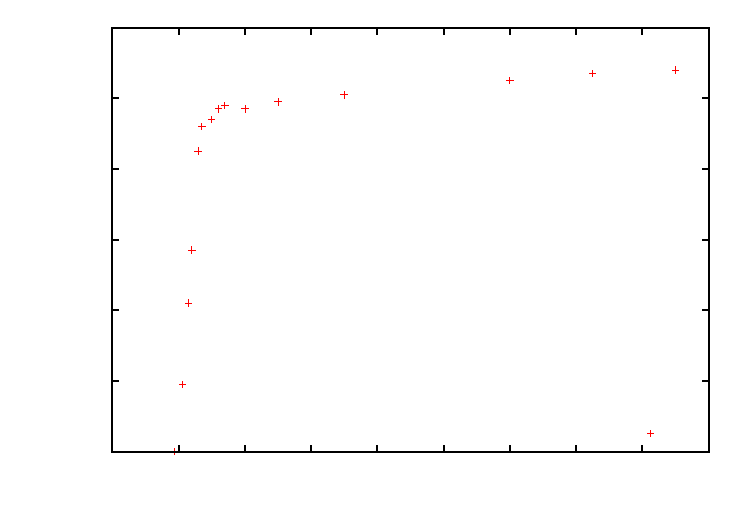
\includegraphics{heiz18}}%
    \gplfronttext
  \end{picture}%
\endgroup

	\caption{Auftragung des Anodenstroms gegen die Anodenspannung bei einem Heizstrom von $I_\text H$=1.8A}
	\label{fig:h18}
\end{figure}
\begin{figure}
	% GNUPLOT: LaTeX picture with Postscript
\begingroup
  \makeatletter
  \providecommand\color[2][]{%
    \GenericError{(gnuplot) \space\space\space\@spaces}{%
      Package color not loaded in conjunction with
      terminal option `colourtext'%
    }{See the gnuplot documentation for explanation.%
    }{Either use 'blacktext' in gnuplot or load the package
      color.sty in LaTeX.}%
    \renewcommand\color[2][]{}%
  }%
  \providecommand\includegraphics[2][]{%
    \GenericError{(gnuplot) \space\space\space\@spaces}{%
      Package graphicx or graphics not loaded%
    }{See the gnuplot documentation for explanation.%
    }{The gnuplot epslatex terminal needs graphicx.sty or graphics.sty.}%
    \renewcommand\includegraphics[2][]{}%
  }%
  \providecommand\rotatebox[2]{#2}%
  \@ifundefined{ifGPcolor}{%
    \newif\ifGPcolor
    \GPcolortrue
  }{}%
  \@ifundefined{ifGPblacktext}{%
    \newif\ifGPblacktext
    \GPblacktexttrue
  }{}%
  % define a \g@addto@macro without @ in the name:
  \let\gplgaddtomacro\g@addto@macro
  % define empty templates for all commands taking text:
  \gdef\gplbacktext{}%
  \gdef\gplfronttext{}%
  \makeatother
  \ifGPblacktext
    % no textcolor at all
    \def\colorrgb#1{}%
    \def\colorgray#1{}%
  \else
    % gray or color?
    \ifGPcolor
      \def\colorrgb#1{\color[rgb]{#1}}%
      \def\colorgray#1{\color[gray]{#1}}%
      \expandafter\def\csname LTw\endcsname{\color{white}}%
      \expandafter\def\csname LTb\endcsname{\color{black}}%
      \expandafter\def\csname LTa\endcsname{\color{black}}%
      \expandafter\def\csname LT0\endcsname{\color[rgb]{1,0,0}}%
      \expandafter\def\csname LT1\endcsname{\color[rgb]{0,1,0}}%
      \expandafter\def\csname LT2\endcsname{\color[rgb]{0,0,1}}%
      \expandafter\def\csname LT3\endcsname{\color[rgb]{1,0,1}}%
      \expandafter\def\csname LT4\endcsname{\color[rgb]{0,1,1}}%
      \expandafter\def\csname LT5\endcsname{\color[rgb]{1,1,0}}%
      \expandafter\def\csname LT6\endcsname{\color[rgb]{0,0,0}}%
      \expandafter\def\csname LT7\endcsname{\color[rgb]{1,0.3,0}}%
      \expandafter\def\csname LT8\endcsname{\color[rgb]{0.5,0.5,0.5}}%
    \else
      % gray
      \def\colorrgb#1{\color{black}}%
      \def\colorgray#1{\color[gray]{#1}}%
      \expandafter\def\csname LTw\endcsname{\color{white}}%
      \expandafter\def\csname LTb\endcsname{\color{black}}%
      \expandafter\def\csname LTa\endcsname{\color{black}}%
      \expandafter\def\csname LT0\endcsname{\color{black}}%
      \expandafter\def\csname LT1\endcsname{\color{black}}%
      \expandafter\def\csname LT2\endcsname{\color{black}}%
      \expandafter\def\csname LT3\endcsname{\color{black}}%
      \expandafter\def\csname LT4\endcsname{\color{black}}%
      \expandafter\def\csname LT5\endcsname{\color{black}}%
      \expandafter\def\csname LT6\endcsname{\color{black}}%
      \expandafter\def\csname LT7\endcsname{\color{black}}%
      \expandafter\def\csname LT8\endcsname{\color{black}}%
    \fi
  \fi
  \setlength{\unitlength}{0.0500bp}%
  \begin{picture}(7200.00,5040.00)%
    \gplgaddtomacro\gplbacktext{%
      \csname LTb\endcsname%
      \put(946,704){\makebox(0,0)[r]{\strut{} 0}}%
      \put(946,1518){\makebox(0,0)[r]{\strut{} 0.5}}%
      \put(946,2332){\makebox(0,0)[r]{\strut{} 1}}%
      \put(946,3147){\makebox(0,0)[r]{\strut{} 1.5}}%
      \put(946,3961){\makebox(0,0)[r]{\strut{} 2}}%
      \put(946,4775){\makebox(0,0)[r]{\strut{} 2.5}}%
      \put(1078,484){\makebox(0,0){\strut{}-20}}%
      \put(1714,484){\makebox(0,0){\strut{} 0}}%
      \put(2350,484){\makebox(0,0){\strut{} 20}}%
      \put(2986,484){\makebox(0,0){\strut{} 40}}%
      \put(3622,484){\makebox(0,0){\strut{} 60}}%
      \put(4259,484){\makebox(0,0){\strut{} 80}}%
      \put(4895,484){\makebox(0,0){\strut{} 100}}%
      \put(5531,484){\makebox(0,0){\strut{} 120}}%
      \put(6167,484){\makebox(0,0){\strut{} 140}}%
      \put(6803,484){\makebox(0,0){\strut{} 160}}%
      \put(176,2739){\rotatebox{-270}{\makebox(0,0){\strut{}Anodenstrom $I_\text A \; [A]$}}}%
      \put(3940,154){\makebox(0,0){\strut{}Spannung U $[V]$}}%
    }%
    \gplgaddtomacro\gplfronttext{%
      \csname LTb\endcsname%
      \put(5816,877){\makebox(0,0)[r]{\strut{}$I_\text{H}=1.9$A}}%
    }%
    \gplbacktext
    \put(0,0){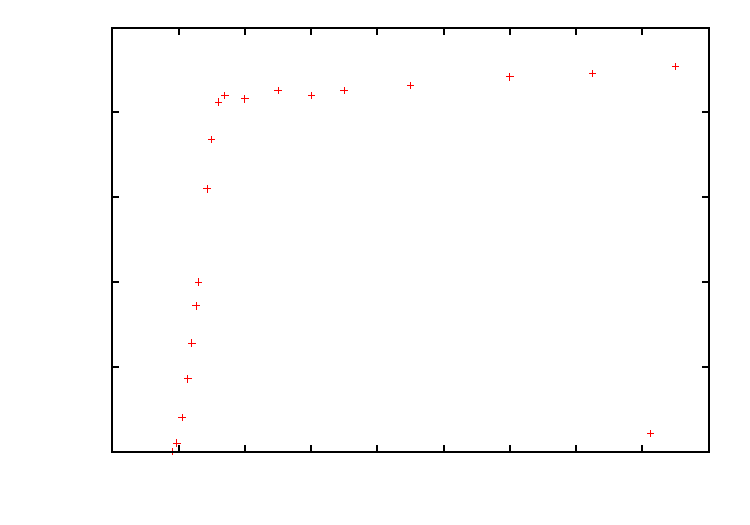
\includegraphics{heiz19}}%
    \gplfronttext
  \end{picture}%
\endgroup

	\caption{Auftragung des Anodenstroms gegen die Anodenspannung bei einem Heizstrom von $I_\text H$=1.9A}
	\label{fig:h19}
\end{figure}
\begin{figure}
	% GNUPLOT: LaTeX picture with Postscript
\begingroup
  \makeatletter
  \providecommand\color[2][]{%
    \GenericError{(gnuplot) \space\space\space\@spaces}{%
      Package color not loaded in conjunction with
      terminal option `colourtext'%
    }{See the gnuplot documentation for explanation.%
    }{Either use 'blacktext' in gnuplot or load the package
      color.sty in LaTeX.}%
    \renewcommand\color[2][]{}%
  }%
  \providecommand\includegraphics[2][]{%
    \GenericError{(gnuplot) \space\space\space\@spaces}{%
      Package graphicx or graphics not loaded%
    }{See the gnuplot documentation for explanation.%
    }{The gnuplot epslatex terminal needs graphicx.sty or graphics.sty.}%
    \renewcommand\includegraphics[2][]{}%
  }%
  \providecommand\rotatebox[2]{#2}%
  \@ifundefined{ifGPcolor}{%
    \newif\ifGPcolor
    \GPcolortrue
  }{}%
  \@ifundefined{ifGPblacktext}{%
    \newif\ifGPblacktext
    \GPblacktexttrue
  }{}%
  % define a \g@addto@macro without @ in the name:
  \let\gplgaddtomacro\g@addto@macro
  % define empty templates for all commands taking text:
  \gdef\gplbacktext{}%
  \gdef\gplfronttext{}%
  \makeatother
  \ifGPblacktext
    % no textcolor at all
    \def\colorrgb#1{}%
    \def\colorgray#1{}%
  \else
    % gray or color?
    \ifGPcolor
      \def\colorrgb#1{\color[rgb]{#1}}%
      \def\colorgray#1{\color[gray]{#1}}%
      \expandafter\def\csname LTw\endcsname{\color{white}}%
      \expandafter\def\csname LTb\endcsname{\color{black}}%
      \expandafter\def\csname LTa\endcsname{\color{black}}%
      \expandafter\def\csname LT0\endcsname{\color[rgb]{1,0,0}}%
      \expandafter\def\csname LT1\endcsname{\color[rgb]{0,1,0}}%
      \expandafter\def\csname LT2\endcsname{\color[rgb]{0,0,1}}%
      \expandafter\def\csname LT3\endcsname{\color[rgb]{1,0,1}}%
      \expandafter\def\csname LT4\endcsname{\color[rgb]{0,1,1}}%
      \expandafter\def\csname LT5\endcsname{\color[rgb]{1,1,0}}%
      \expandafter\def\csname LT6\endcsname{\color[rgb]{0,0,0}}%
      \expandafter\def\csname LT7\endcsname{\color[rgb]{1,0.3,0}}%
      \expandafter\def\csname LT8\endcsname{\color[rgb]{0.5,0.5,0.5}}%
    \else
      % gray
      \def\colorrgb#1{\color{black}}%
      \def\colorgray#1{\color[gray]{#1}}%
      \expandafter\def\csname LTw\endcsname{\color{white}}%
      \expandafter\def\csname LTb\endcsname{\color{black}}%
      \expandafter\def\csname LTa\endcsname{\color{black}}%
      \expandafter\def\csname LT0\endcsname{\color{black}}%
      \expandafter\def\csname LT1\endcsname{\color{black}}%
      \expandafter\def\csname LT2\endcsname{\color{black}}%
      \expandafter\def\csname LT3\endcsname{\color{black}}%
      \expandafter\def\csname LT4\endcsname{\color{black}}%
      \expandafter\def\csname LT5\endcsname{\color{black}}%
      \expandafter\def\csname LT6\endcsname{\color{black}}%
      \expandafter\def\csname LT7\endcsname{\color{black}}%
      \expandafter\def\csname LT8\endcsname{\color{black}}%
    \fi
  \fi
  \setlength{\unitlength}{0.0500bp}%
  \begin{picture}(7200.00,5040.00)%
    \gplgaddtomacro\gplbacktext{%
      \csname LTb\endcsname%
      \put(946,704){\makebox(0,0)[r]{\strut{} 0}}%
      \put(946,1111){\makebox(0,0)[r]{\strut{} 0.5}}%
      \put(946,1518){\makebox(0,0)[r]{\strut{} 1}}%
      \put(946,1925){\makebox(0,0)[r]{\strut{} 1.5}}%
      \put(946,2332){\makebox(0,0)[r]{\strut{} 2}}%
      \put(946,2740){\makebox(0,0)[r]{\strut{} 2.5}}%
      \put(946,3147){\makebox(0,0)[r]{\strut{} 3}}%
      \put(946,3554){\makebox(0,0)[r]{\strut{} 3.5}}%
      \put(946,3961){\makebox(0,0)[r]{\strut{} 4}}%
      \put(946,4368){\makebox(0,0)[r]{\strut{} 4.5}}%
      \put(946,4775){\makebox(0,0)[r]{\strut{} 5}}%
      \put(1078,484){\makebox(0,0){\strut{}-20}}%
      \put(1714,484){\makebox(0,0){\strut{} 0}}%
      \put(2350,484){\makebox(0,0){\strut{} 20}}%
      \put(2986,484){\makebox(0,0){\strut{} 40}}%
      \put(3622,484){\makebox(0,0){\strut{} 60}}%
      \put(4259,484){\makebox(0,0){\strut{} 80}}%
      \put(4895,484){\makebox(0,0){\strut{} 100}}%
      \put(5531,484){\makebox(0,0){\strut{} 120}}%
      \put(6167,484){\makebox(0,0){\strut{} 140}}%
      \put(6803,484){\makebox(0,0){\strut{} 160}}%
      \put(176,2739){\rotatebox{-270}{\makebox(0,0){\strut{}Anodenstrom $I_\text A \; [A]$}}}%
      \put(3940,154){\makebox(0,0){\strut{}Spannung U $[V]$}}%
    }%
    \gplgaddtomacro\gplfronttext{%
      \csname LTb\endcsname%
      \put(5816,877){\makebox(0,0)[r]{\strut{}$I_\text{H}=\SI{2.0}{\ampere}$}}%
    }%
    \gplbacktext
    \put(0,0){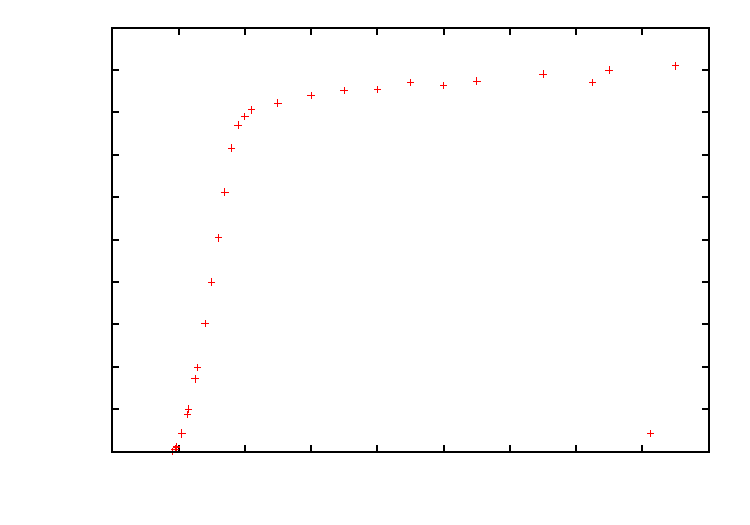
\includegraphics{heiz2}}%
    \gplfronttext
  \end{picture}%
\endgroup

	\caption{Auftragung des Anodenstroms gegen die Anodenspannung bei einem Heizstrom von $I_\text H$=2A}
	\label{fig:h2}
\end{figure}
\begin{figure}
	% GNUPLOT: LaTeX picture with Postscript
\begingroup
  \makeatletter
  \providecommand\color[2][]{%
    \GenericError{(gnuplot) \space\space\space\@spaces}{%
      Package color not loaded in conjunction with
      terminal option `colourtext'%
    }{See the gnuplot documentation for explanation.%
    }{Either use 'blacktext' in gnuplot or load the package
      color.sty in LaTeX.}%
    \renewcommand\color[2][]{}%
  }%
  \providecommand\includegraphics[2][]{%
    \GenericError{(gnuplot) \space\space\space\@spaces}{%
      Package graphicx or graphics not loaded%
    }{See the gnuplot documentation for explanation.%
    }{The gnuplot epslatex terminal needs graphicx.sty or graphics.sty.}%
    \renewcommand\includegraphics[2][]{}%
  }%
  \providecommand\rotatebox[2]{#2}%
  \@ifundefined{ifGPcolor}{%
    \newif\ifGPcolor
    \GPcolortrue
  }{}%
  \@ifundefined{ifGPblacktext}{%
    \newif\ifGPblacktext
    \GPblacktexttrue
  }{}%
  % define a \g@addto@macro without @ in the name:
  \let\gplgaddtomacro\g@addto@macro
  % define empty templates for all commands taking text:
  \gdef\gplbacktext{}%
  \gdef\gplfronttext{}%
  \makeatother
  \ifGPblacktext
    % no textcolor at all
    \def\colorrgb#1{}%
    \def\colorgray#1{}%
  \else
    % gray or color?
    \ifGPcolor
      \def\colorrgb#1{\color[rgb]{#1}}%
      \def\colorgray#1{\color[gray]{#1}}%
      \expandafter\def\csname LTw\endcsname{\color{white}}%
      \expandafter\def\csname LTb\endcsname{\color{black}}%
      \expandafter\def\csname LTa\endcsname{\color{black}}%
      \expandafter\def\csname LT0\endcsname{\color[rgb]{1,0,0}}%
      \expandafter\def\csname LT1\endcsname{\color[rgb]{0,1,0}}%
      \expandafter\def\csname LT2\endcsname{\color[rgb]{0,0,1}}%
      \expandafter\def\csname LT3\endcsname{\color[rgb]{1,0,1}}%
      \expandafter\def\csname LT4\endcsname{\color[rgb]{0,1,1}}%
      \expandafter\def\csname LT5\endcsname{\color[rgb]{1,1,0}}%
      \expandafter\def\csname LT6\endcsname{\color[rgb]{0,0,0}}%
      \expandafter\def\csname LT7\endcsname{\color[rgb]{1,0.3,0}}%
      \expandafter\def\csname LT8\endcsname{\color[rgb]{0.5,0.5,0.5}}%
    \else
      % gray
      \def\colorrgb#1{\color{black}}%
      \def\colorgray#1{\color[gray]{#1}}%
      \expandafter\def\csname LTw\endcsname{\color{white}}%
      \expandafter\def\csname LTb\endcsname{\color{black}}%
      \expandafter\def\csname LTa\endcsname{\color{black}}%
      \expandafter\def\csname LT0\endcsname{\color{black}}%
      \expandafter\def\csname LT1\endcsname{\color{black}}%
      \expandafter\def\csname LT2\endcsname{\color{black}}%
      \expandafter\def\csname LT3\endcsname{\color{black}}%
      \expandafter\def\csname LT4\endcsname{\color{black}}%
      \expandafter\def\csname LT5\endcsname{\color{black}}%
      \expandafter\def\csname LT6\endcsname{\color{black}}%
      \expandafter\def\csname LT7\endcsname{\color{black}}%
      \expandafter\def\csname LT8\endcsname{\color{black}}%
    \fi
  \fi
  \setlength{\unitlength}{0.0500bp}%
  \begin{picture}(7200.00,5040.00)%
    \gplgaddtomacro\gplbacktext{%
      \csname LTb\endcsname%
      \put(946,704){\makebox(0,0)[r]{\strut{} 0}}%
      \put(946,1111){\makebox(0,0)[r]{\strut{} 0.5}}%
      \put(946,1518){\makebox(0,0)[r]{\strut{} 1}}%
      \put(946,1925){\makebox(0,0)[r]{\strut{} 1.5}}%
      \put(946,2332){\makebox(0,0)[r]{\strut{} 2}}%
      \put(946,2740){\makebox(0,0)[r]{\strut{} 2.5}}%
      \put(946,3147){\makebox(0,0)[r]{\strut{} 3}}%
      \put(946,3554){\makebox(0,0)[r]{\strut{} 3.5}}%
      \put(946,3961){\makebox(0,0)[r]{\strut{} 4}}%
      \put(946,4368){\makebox(0,0)[r]{\strut{} 4.5}}%
      \put(946,4775){\makebox(0,0)[r]{\strut{} 5}}%
      \put(1078,484){\makebox(0,0){\strut{}-20}}%
      \put(1714,484){\makebox(0,0){\strut{} 0}}%
      \put(2350,484){\makebox(0,0){\strut{} 20}}%
      \put(2986,484){\makebox(0,0){\strut{} 40}}%
      \put(3622,484){\makebox(0,0){\strut{} 60}}%
      \put(4259,484){\makebox(0,0){\strut{} 80}}%
      \put(4895,484){\makebox(0,0){\strut{} 100}}%
      \put(5531,484){\makebox(0,0){\strut{} 120}}%
      \put(6167,484){\makebox(0,0){\strut{} 140}}%
      \put(6803,484){\makebox(0,0){\strut{} 160}}%
      \put(176,2739){\rotatebox{-270}{\makebox(0,0){\strut{}Anodenstrom $I_\text A \; [A]$}}}%
      \put(3940,154){\makebox(0,0){\strut{}Spannung U $[V]$}}%
    }%
    \gplgaddtomacro\gplfronttext{%
      \csname LTb\endcsname%
      \put(5816,4602){\makebox(0,0)[r]{\strut{}$I_\text{H}=2$A}}%
      \csname LTb\endcsname%
      \put(5816,4382){\makebox(0,0)[r]{\strut{}$I_\text{H}=1.9$A}}%
      \csname LTb\endcsname%
      \put(5816,4162){\makebox(0,0)[r]{\strut{}$I_\text{H}=1.8$A}}%
    }%
    \gplbacktext
    \put(0,0){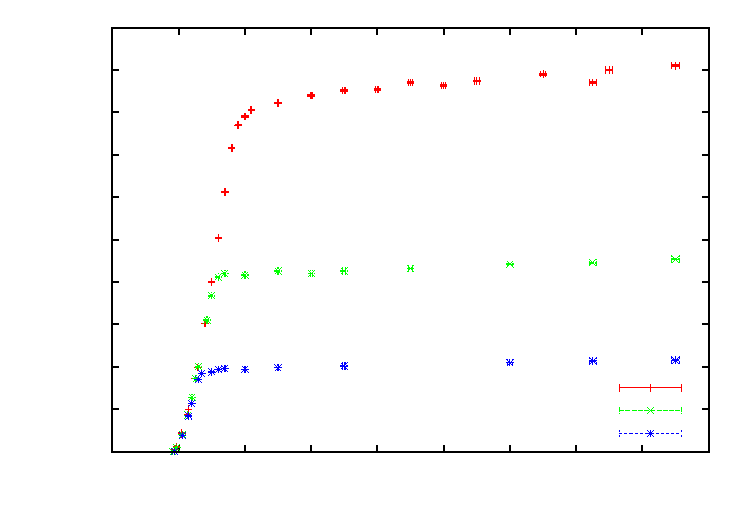
\includegraphics{heiz}}%
    \gplfronttext
  \end{picture}%
\endgroup

	\caption{Auftragung des Anodenstroms gegen die Anodenspannung bei unterschiedlichen Heizströmen}
	\label{fig:h}
\end{figure}

\section{Diskussion}
\label{sec:diskussion}

\bibliography{literatur}
\bibliographystyle{babalpha}
\end{document}
